%% V1.0
%% by Gabriel Garcia, gabrcg@gmail.com
%% This is a template for Udacity projects using IEEEtran.cls

%% Be Udacious!

\documentclass[10pt,journal,compsoc]{IEEEtran}

    \usepackage[pdftex]{graphicx}    
    \usepackage{cite}
    \hyphenation{op-tical net-works semi-conduc-tor}
    
    
    \begin{document}
    
    \title{Deep Learning guinea pig image classification using NVidia DIGITS and GoogLeNet}
    
    \author{\textbf{Lukasz Zmudzinski} \\ University of Warmia and Mazury in Olsztyn \\ lukasz@zmudzinski.me}
    
    %\markboth{Inference project, Robotic Nanodegree, Udacity}%
    %{}
    \IEEEtitleabstractindextext{%
    
    \begin{abstract}
    In this paper guinea pig classification using deep learning imaging methods was performed on the Nvidia DIGITS 6. Models capable of distinguishing skinny, abyssinian and crested fur types were created in the process. To increase the classification accuracy empty images (with only the background) were added to the data set. Upon evaluation, the created model recognized the animals correctly from images taken in various household backgrounds.
    \end{abstract}
    
    % Note that keywords are not normally used for peerreview papers.
    \begin{IEEEkeywords}
    classification, deep learning, animal recognition, robotics, DIGITS.
    \end{IEEEkeywords}}
    
    
    \maketitle
    \IEEEdisplaynontitleabstractindextext
    \IEEEpeerreviewmaketitle
    \section{Introduction}
    \label{sec:introduction}
    
    \IEEEPARstart{R}{obotic} systems are nowadays increasingly introduced in various animal care facilities like farms, daries and shelters \cite{agrirobo, dairyrobo}. With the growing need of automating work more methods of image classification and decision making are needed. 

    In this work, deep learning techniques were utilized to create a classification model of guinea pigs in different home environments, to explore the possibilities of bringing such systems into the world of household animals.
    
    %example for inserting image
    %\begin{figure}[thpb]
    %      \centering
    %      \caption{Robot Revolution.}
    %      \label{fig:robot1}
    %\end{figure}
    
    \subsection{Nvidia DIGITS}
    DIGITS (NVIDIA Deep Learning GPU Training System) was used in this project. It allows to rapidly train deep neural networks (DNNs) for image classification, segmentation and object detection tasks \cite{digitswww}. \newline\newline
    The solution comes with pre-trained models for example:

    \begin{itemize}
        \item GoogLeNet,
        \item AlexNet,
        \item UNET and more.        
    \end{itemize}
    \noindent
    In this paper GoogLeNet was used as the model of choice.
    
    \section{Background / Formulation}
    Deep Learning is growing in popularity over the past few years. It is connected to the fact that it becomes more useful than before thanks to the amount of available training data and advances in computer hardware/software \cite{dl}. 

    Another problem with neural networks in general was vanishing gradients and unpredictable weight initialization \cite{glnp}. This becomes solved by the use of RELUs (Rectified Linear Units)\cite{relu} and more recently the GoogLeNet deep learning model\cite{dwc}.

    In neural network algorithms we can tweak several parameters, that will greately impact the final output: number of epochs, learning rate, solver type and many more.

    \begin{itemize}
        \item \textbf{Epoch} - one complete pass  of the data in the data set. The amount of epochs should be determined through tests. Small number of epochs often leads to bad predictions, while a big number leads to overfitting.
        \item \textbf{Learning rate} - describes the rate at which the network abandons old beliefs, for new ones to take their place. The value must be correct, values that are too big or too small may lead to bad predictions.
        \item \textbf{Solver type} - contains information about how the weights are updated for the network. This project used one of the most popular ones: Stochastic Gradient Descent (SGD) \cite{sgd}. 
    \end{itemize}

    GoogLeNet connects various techniques known from Deep Learning like convolutions, pooling, adding softmax and more, to distinguish all the objects that are present in the image. 

    \section{Data Acquisition}
    The data was collected by recording a square video of each guinea pig over a period of 30 seconds in different environments and then extracting each frame as an image. Each frame was then lowered in resolution to 256px in order to fit GoogLeNet requirements. Example images can be seen in Fig. \ref{fig:pigs}.
    \newline\newline
    To ensure good accuracy of the model, each set had to cover front, side and back angles of the guinea pig body. Moreover empty images (without guinea pigs) were added of the provided backgrounds, to increase classification accuracy (and to distinguish background from objects that should be recognized).
    \newline\newline
    Guinea pigs used in the experiment:

    \begin{itemize}
        \item Fifi (4 years, abyssinian),
        \item Rey (2 years, crested),
        \item Asajj (2 years, skinny).
    \end{itemize}

    \noindent Using the data, four labels were produced and assigned to the following neural network classes:

    \begin{itemize}
        \item \textbf{None} - when there is no guinea pig in the image,
        \item \textbf{Ayssinian}, \textbf{Crested} and \textbf{Skinny} - fur type.
    \end{itemize}

    \begin{figure}[h]
        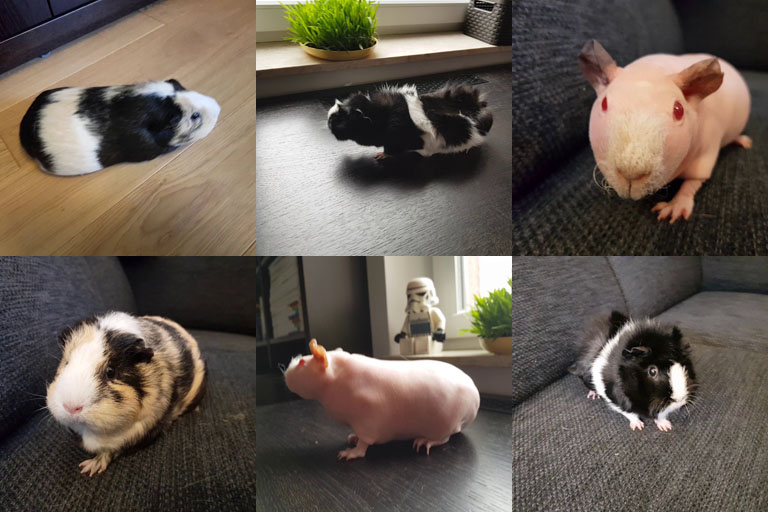
\includegraphics[width=\linewidth]{pig_dataset.png}
        \caption{Example images for abyssinian, crested and skinny guinea pigs from the provided data set.}
        \label{fig:pigs}
        \centering
    \end{figure}
    
    \section{Results}

    The final classification model was gathered from running the described image set over 15 epochs of GoogLeNet model on Nvidia DIGITS. As you can see on Fig. \ref{fig:googlenet} the accuracy after 15 epochs rose to over $90\%$, while the finall value loss was around $0.3$ with a learning rate of $0.01$. Using more epochs and a different learning was tested, but it led to overfitting of the data.

    \begin{figure}[h]
        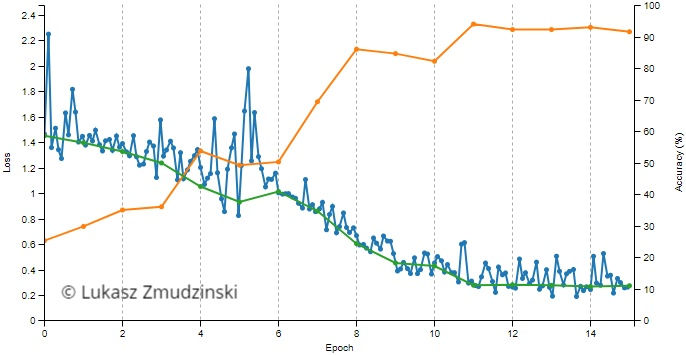
\includegraphics[width=\linewidth]{googlenet.png}
        \caption{Graph showing the value accuracy (orange), test data loss (blue) and value loss (green) after running the GoogLeNet model.}
        \label{fig:googlenet}
        \centering
    \end{figure}

    After the model was created, a series of tests were performed to check, if the inference is correct. The first set of tests consisted of images from the previously gathered data set. The prediction was always right for provided images, with the value between 70\%-95\%. You can see an example result on Fig. \ref{fig:result_01}.
    
    \begin{figure}[h]
        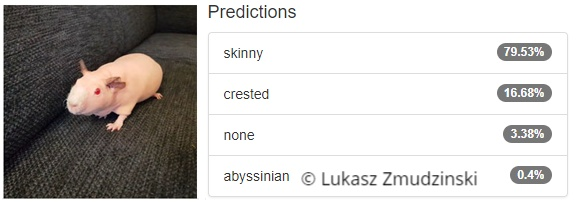
\includegraphics[width=\linewidth]{result_01.png}
        \caption{Example correct prediction results (79.53\%) using previously captured images in selected environments using GoogLeNet.}
        \label{fig:result_01}
        \centering
    \end{figure}

    After acquiring enough information on the predictions, tests on new images were performed (different environments, same guinea pigs) giving satisfactory results - guinea pigs were classified correctly on each provided picture containing the animal. Example result on Fig. \ref{fig:result_02}.

    One failed prediction was encountered, when a picture of a background with a cat was used. The cat was badly classified as an abyssinian guinea pig.

    \begin{figure}[h]
        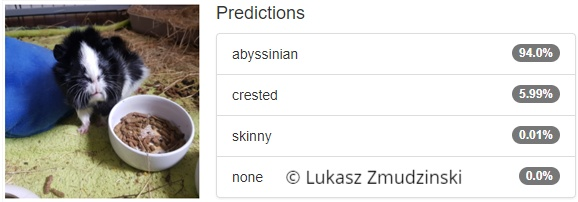
\includegraphics[width=\linewidth]{result_02.png}
        \caption{Example correct prediction results (94.0\%) using post-model captured images in animal cage environment using GoogLeNet.}
        \label{fig:result_02}
        \centering
    \end{figure}
    
    \section{Discussion}
    TODO
    
    \section{Conclusion / Future work}
    The created model proves that guinea pig fur recognition for robotic systems is possible. The project gave good results - the created model recognized the animals correctly from images taken in various household backgrounds. The prediction was acquired fast (under 5ms) making the inference time low. This is especially important for robotic systems that deal with live animals, because the reaction times need to be rapid. \newline\newline
    Future work might include robotic systems that monitor the state of specific animals, adjust food distribution depending on image readings or alert when the guinea pig suffers from any kind of illness.
    
   \bibliography{bib}
   \bibliographystyle{ieeetr}
    
    \end{document}